\chapter{Research, Enterprise, and Domain-Specific Agent Systems}\label{ch:C24}
The 2026 Knowledge Activation study and ALE locate two different evidence boundaries. The former reports engineers' perceived benefits in a particular organizational study; the latter constructs professional task evaluations whose measured outcomes do not directly identify enterprise productivity or economy-wide value~\cite{corpus260314805,corpus260605405}. Treating either as proof that a named product improves every knowledge workflow would exceed its design. This chapter uses those boundaries to connect source-grounded research, permissioned business effects, memory services, and the deployment experiments required to establish value.

Research and enterprise agents share an evidence problem but differ in what their outputs authorize. A research agent must connect conclusions to sources and preserve unresolved disagreement. An enterprise agent may use those conclusions to change a customer record, create a legal work product, or trigger a business process. The latter adds identity, permissions, transactional effects, and organizational accountability. A fluent report is insufficient evidence for either role, and a well-grounded report does not automatically authorize the actions it recommends.

The objective of this chapter is a role-based account of these systems, including memory services that supply their context. Product documentation identifies integration and execution surfaces available for inspection; it does not establish scientific validity, deployment benefit, or universal capability. The analysis therefore connects each family to a concrete failure mechanism and a discriminating evaluation.

\section{Research as evidence acquisition and revision}\label{sec:C24:research}
A research workflow contains query construction, source acquisition, identity resolution, claim extraction, comparison, synthesis, and revision. Each stage can fail independently. A source can be relevant but outdated, a claim can be extracted accurately but applied to the wrong population, or a synthesis can cite a paper that never measured the asserted outcome. Counting citations or generated pages does not distinguish these errors.

Represent a claim as a tuple containing proposition, scope, evidence class, source version, result location, assumptions, and unresolved limitations. An evidence graph links claims to supporting or contradicting observations. This representation makes revision possible: if a paper changes its result, the system can identify dependent conclusions rather than rewrite every paragraph blindly. It also separates author-reported evidence from independent reproduction and analytical deduction.

The query policy should seek disconfirming evidence as well as support. A system rewarded for completing a coherent report can stop after finding sources that fit its initial hypothesis. A better evaluation includes questions where the decisive result is negative, where two studies use incompatible definitions, or where the available implementation cannot substantiate a headline claim. The correct output may be a narrower conclusion or an explicit unresolved state rather than a more confident answer.

Hosted research products and inspectable research harnesses occupy different reproducibility boundaries. DeerFlow exposes a research-oriented harness, while Asta's public resources distinguish research implementations from the hosted service~\cite{executionproduct029,executionproduct058}. Consequently, a result obtained with a published baseline cannot be attributed to every hosted variant, and a hosted demonstration does not reproduce the baseline. Evaluation must name the actual execution path and available tools.

The stopping condition is evidence sufficiency under a declared question, not exhaustion of a token budget or attainment of a target report length. An implementation can maintain unresolved claim categories and a bounded search frontier. It should report whether searches failed because no qualifying evidence was found, because a source was inaccessible, or because the budget ended. These states have different scientific implications and should not collapse into a single statement that evidence is absent.

\subsection{Biological agents: executable methods and empirical feedback}\label{sec:C24:biology}
The October 2026 biological frontier spans several distinct control loops. Paper2Agent converts papers and associated code into MCP interfaces and checks their executable behavior; its September Nature article demonstrates genomic and transcriptomic cases while retaining human responsibility for open-ended interpretation~\cite{miao2026paper2agent}. WetRobo's September report instead studies coding-agent adaptation of a laboratory robot kit on three equipment-manipulation tasks, including bottle-cap transfer between two laboratories~\cite{oikawa2026wetrobo}. Neither result alone establishes autonomous experimental discovery: method execution, equipment manipulation, scientific interpretation and selection of new experiments are different tasks with different ground truth.

This distinction determines what memory should retain. Reusing a numerical analysis method requires its data schema, software revision and assumptions. Reusing an equipment procedure additionally requires calibration, object geometry, admissible operating conditions and an execution monitor. Reusing a scientific conclusion requires evidence about the sampled biological system and measurement process. A skill that retains only successful command text can erase all three applicability boundaries. Model improvement does not repair a missing calibration record or turn an association into a validated mechanism.

The inspected Paper2Agent revision makes a limited verification boundary concrete. Its \path{validate_cases} routine can require positive acceptance cases for every expected tool; \path{check_subset} compares returned structures with declared expected values; \path{check_artifacts} checks returned artifact paths and identity conditions. Those functions support interface and smoke-case checks, not independent validation of a biological interpretation. The source was inspected at revision \texttt{8c2d059165ef}; no scientific analysis was executed here~\cite{paper2agent2026code}. Generated tests inherit the assumptions of their expected outputs. An executable wrapper can therefore improve method accessibility while faithfully automating an invalid analysis; interface conformance and scientific validity must remain separate claims.

Figure~\ref{fig:C24:scientificloop} locates the evidence and execution boundaries in a conceptual scientific-agent loop.
\begin{figure}[!htbp]
\centering
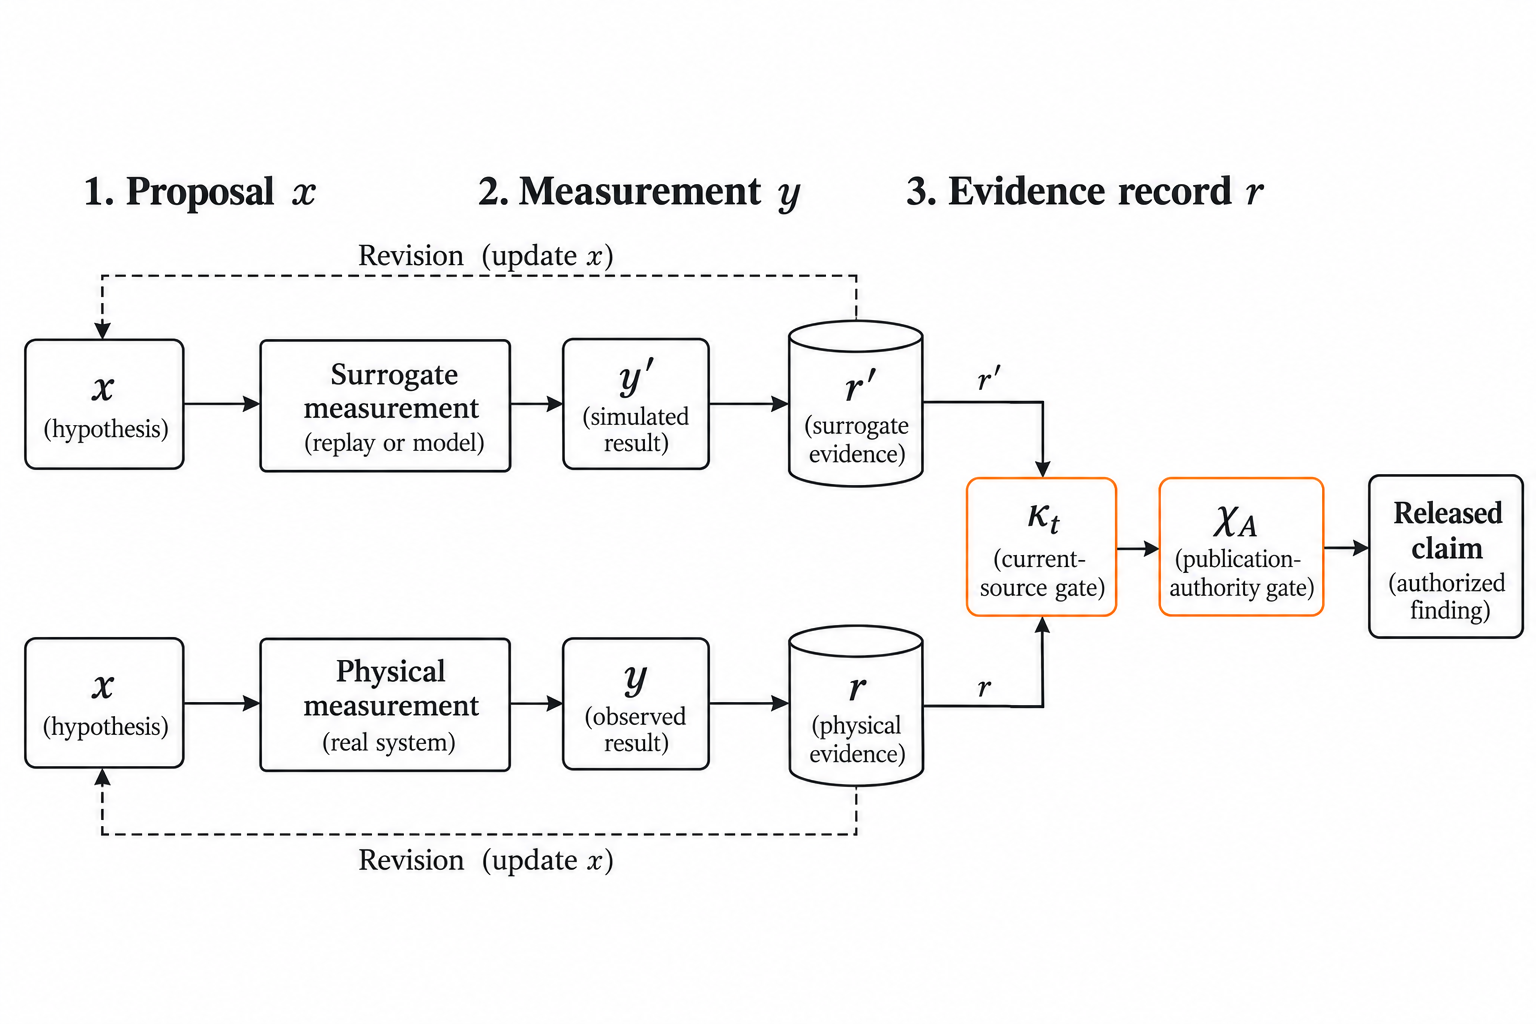
\includegraphics[width=\linewidth]{book/figures/assets/F24review.png}
\caption{Only records already accepted by the declared verifier enter the current-source validity and publication-authority gates. A released surrogate or replay finding retains its backend and recording provenance; it is not fresh physical evidence. Closing either loop does not identify a causal improvement or establish unrestricted laboratory autonomy.}
\label{fig:C24:scientificloop}
\end{figure}

\subsection{An October closed-loop result and its attribution limits}
Cutts and colleagues report three agent-guided aptamer design--test--improve rounds in October 2026~\cite{cutts2026aptamers}. The myoglobin results in Table~\ref{tab:C24:aptamers} are nonmonotonic across rounds. Human researchers performed the laboratory workflow, and the agent platform changed after the first round. The study therefore provides empirical evidence of iterative laboratory feedback and failure diagnosis, while its authors explicitly reserve matched-budget no-feedback and non-reasoning controls for future work. These observations do not isolate the causal contribution of agentic reasoning from harness changes, prior-round seeds or accumulated assay information.

\begingroup\setlength{\tabcolsep}{4pt}\small
\begin{table}[!htbp]
\centering
\caption{Author-reported bead-corrected myoglobin hits among newly designed primary candidates. Candidate populations differ across rounds; these are campaign observations, not randomized treatment-effect estimates. Source: Results R.2 of Cutts et al.~\cite{cutts2026aptamers}.}
\label{tab:C24:aptamers}
\begin{tabular}{lrrr}
\toprule Round & Hits & Candidates & Hit rate (\%) \\
\midrule
1 & 20 & 196 & 10.2 \\
2 & 9 & 244 & 3.7 \\
3 & 184 & 549 & 33.5 \\
\bottomrule
\end{tabular}
\end{table}
\endgroup

The nonmonotonic middle round is analytically important. Optimizing an assay proxy can concentrate candidates in a region with favorable background interactions rather than the desired biological property. A memory writer that records only the apparent successful motif can promote the shortcut into a procedural prior. A writer that retains target and background evidence, candidate lineage, analysis revision and uncertainty makes the lesson revisable. This is the biological counterpart of a coding agent memorizing a test-specific patch: a higher proxy score can accompany weaker alignment with the actual objective.

For a transparent analysis, consider the illustrative measurement model
\begin{align}
 y_{rk}&=f(x_{rk},e_r)+b_{p(r,k)}+\varepsilon_{rk},\\
 \mathbb E[\varepsilon_{rk}\mid x_{rk},e_r,p(r,k)]&=0.
\end{align}
Here $x_{rk}$ is candidate $k$ in round $r$, $e_r$ the declared assay conditions, $p(r,k)$ its measurement batch, $b_p$ a batch effect, and $y_{rk}$ the observed scalar response; all additive terms have the response's units. This is an analytical model, not a fitted model of the cited experiment. If candidate strategy changes only between batches, differences in $f$ and $b_p$ are not separately identified without additional design or assumptions. Randomized allocation within batches, recurring controls, replicated candidates and independent confirmation can address different parts of that ambiguity. Repeated reads of one construct are measurement replication; they do not create independent evidence about unrelated molecular families.

An agent-design comparison must therefore randomize complete campaigns or sufficiently isolated candidate allocations, preserve assay conditions and measurement budgets, and predeclare which feedback is available before each proposal. Include conventional sequential-design and no-feedback controls, not only a weak language-model prompt. Hold out candidate families or experimental regimes when the claim concerns transfer. Evaluate the selected designs and the learned predictor separately: finding a promising candidate and predicting unseen candidates are different achievements. Costs include physical measurements, waiting, failed jobs, analyst review and computational selection. Token expenditure alone is an inadequate resource boundary when empirical feedback dominates elapsed time.

\subsection{Replay laboratories, digital twins and live measurements}
Autonomous Science Bench, released in October 2026, makes that discovery--learning distinction explicit through two acceptance gates~\cite{wen2026asbench}. Version 0.1 contains six campaigns: five return recorded measurements and one uses a hidden surrogate. A live backend and adaptive allocation scheduler are planned, rather than evaluated results in that release. The laboratory service owns the measurement ledger independently of the agent, and grading combines measured-design quality with prediction on held-out designs. These design choices support controlled evaluation of sequential decisions; they do not constitute six live autonomous laboratory demonstrations.

The backend is part of the scientific claim. A replay can provide genuine historical measurements while excluding unrecorded designs. A digital twin permits more queries but tests optimization against its approximation and training coverage. A live assay adds drift, failed measurements, delayed returns and limits on reversibility. An interface that makes those backends look identical to the agent does not make their evidence interchangeable. Report backend provenance with every outcome and measure whether an agent exploits surrogate artifacts that fail under independent measurement.

Biological scope also constrains the autonomy claim. The aptamer study uses non-infectious protein targets under its stated laboratory conditions and does not study clinical efficacy, human subjects, or animal models~\cite{cutts2026aptamers}. An assay hit therefore remains an assay-specific observation. Extending a workflow to a different biological system requires its own material, measurement, containment, and approval conditions; preserving an API schema supplies none of those premises. The relevant system boundary includes the people or equipment that accept a proposed experiment and the independent evidence required before a scientific conclusion is promoted.

Delayed results create a further state boundary. Submitted, measured, quality-controlled and scientifically accepted experiments should have distinct identifiers and statuses. An agent must not treat an unreturned measurement as a negative label or spend the same physical budget twice after a timeout. When a result is corrected, dependent hypotheses and skills become stale without erasing the historical reason for their adoption. These requirements connect biological research to the session journal of Chapter~\ref{ch:C13}, the conditioning analysis of Chapter~\ref{ch:C17} and the recovery contracts of Chapter~\ref{ch:C32}. The cross-domain synthesis concerns preservation of evidence, authority and effect identity; it does not imply that software verifiers and biological assays have equivalent error models.

\section{Enterprise grounding and permission propagation}\label{sec:C24:enterprise}
Enterprise context is governed by principals, groups, purpose, retention, and changing access policy. Retrieval must enforce these constraints at use time. A document indexed while a user had access may become unauthorized later. An embedding or extracted summary can preserve sensitive information after the original file is removed. Therefore permission checks cannot be limited to the connector's initial ingestion step.

Let a retrieved record carry source identity $d$, subject $u$, validity interval, and authorization epoch $a$. Before the record enters $C_t$, the application evaluates whether the current principal may use $d$ for the requested purpose under the current epoch. A cached positive decision is reusable only within the policy's declared validity conditions. The record's textual content cannot grant its own authority. Instructions discovered inside a document remain data unless promoted through an authorized application channel.

Business workflow agents also depend on schema and process state. A customer-service action can be valid for one account tier and invalid for another. A procurement step may require approval after a threshold is crossed. These constraints should be represented in tool preconditions and authoritative business logic. Asking the language model to remember all exceptions from a policy manual creates an avoidable single point of failure.

Platforms such as Agentforce, ServiceNow's agent tooling, SAP Joule Studio, and Copilot Studio document domain-integrated development surfaces~\cite{executionproduct045,executionproduct046,executionproduct081,executionproduct072}. The transferable technical question is how those surfaces preserve identity and process constraints across model decisions, connectors, and human review. Their domain integration does not establish that every generated action is correct, nor that all deployment configurations enforce the same controls.

A discriminating test changes access or process state midway through a session. The agent previously read a document or prepared an action, then the principal loses access or the business object changes. Evaluate whether retrieval, pending approvals, and queued actions are invalidated appropriately. A successful fresh-session test is insufficient because the failure lives in stale context and in-flight work. Report benign task completion alongside containment to expose overblocking as well as unauthorized use.


\section{Memory engines are distinct policy components}\label{sec:C24:memoryproducts}
A memory engine can store raw events, extract facts, build a graph, summarize experience, or expose reflection operations. These are distinct mechanisms. Storing more information can improve coverage while increasing retrieval noise and governance burden. A graph can encode temporal relationships without guaranteeing that the selected facts remain valid. A reflection operation can produce a useful abstraction or reinforce a mistaken interpretation.

Mem0, Graphiti/Zep, Hindsight, MemOS, and OpenViking expose different storage and context-management surfaces~\cite{executionproduct024,executionproduct033,executionproduct040,executionproduct083,executionproduct084}. The comparison should identify the unit written, retrieval policy, update semantics, provenance, deletion propagation, and compatibility with the consuming model. A memory product's use of the word learning does not establish changes to model parameters. The actual update target must be inspected.

Temporal memory requires both event time and system knowledge time. An event can occur on one date and be discovered later. A correction can invalidate a prior belief without making the historical observation disappear. A system that stores only the most recent text may lose the explanation for past decisions; one that stores every version without validity filtering may repeatedly retrieve obsolete facts. The application must define which temporal question it is answering.

Memory evaluation also needs a no-memory baseline and an oracle-retrieval control. The former reveals negative transfer; the latter separates storage and retrieval limitations from downstream interpretation. Construction cost belongs inside the accounting boundary. A memory engine can reduce per-task prompt size while spending substantial inference on extraction, consolidation, or maintenance. Amortization depends on reuse and should be reported as a function of workload, not assumed from one benchmark.

Licensing and inspectability remain artifact-specific. Where a repository's license and additional README restrictions appear inconsistent, record the conflict and avoid an unqualified legal classification. The technical consequence is uncertainty about reuse and deployment, not an inference about enforceability. More importantly for scientific comparison, source visibility should not be confused with an audited implementation. A public memory schema can still omit crucial behavior implemented by a remote service.


\section{Work-product and vertical-system inventory}\label{sec:C24:catalog}
Table~\ref{tab:C24:catalog} completes the catalog with research, business, vertical, and memory systems. It describes the role established by the inspected resource and the evidence needed before accepting a stronger claim. Product families can overlap; the categories organize experimental questions rather than define exclusive market segments. Names and source redirects are preserved without importing prior rankings or unverified ownership assertions.
\begingroup\setlength{\tabcolsep}{3pt}\small
\bookneedspace{.42\textheight}
\begin{longtable}{L{25mm}L{35mm}L{48mm}}
\caption{Research enterprise and memory products with role-specific checks.}\label{tab:C24:catalog}\\
\toprule Product & Inspected role & Diagnostic condition \\
\midrule\endfirsthead
\toprule Product & Inspected role & Diagnostic condition \\
\midrule\endhead
Mem0\cite{executionproduct024} & Fact-oriented memory layer & Test corrections, source provenance and deletion across derived records. \\
DeerFlow\cite{executionproduct029} & Inspectable research harness & Pin search tools and measure contradictory-evidence coverage at matched budget. \\
Graphiti / Zep\cite{executionproduct033} & Temporal graph context & Distinguish event time, knowledge time and invalidated facts during retrieval. \\
watsonx Orchestrate\cite{executionproduct034} & Enterprise orchestration & Verify connector principal propagation and business-process constraints at dispatch. \\
Hindsight\cite{executionproduct040} & Retention recall and reflection & Audit whether reflection adds unsupported inferences or preserves source links. \\
Agentforce\cite{executionproduct045} & CRM-grounded business agents & Change account state mid-run and test action preconditions and approval binding. \\
AI Agent Studio / Otto AI Agents\cite{executionproduct046} & Service-workflow agent tooling & Distinguish workflow completion from successful resolution and absence of adverse effects. \\
ChatGPT Work\cite{executionproduct047} & Research and connected work artifacts & Audit claim support and the exact saved artifact; hosted internals remain opaque. \\
Claude: work and Research\cite{executionproduct048} & Research and file-oriented work & Separate merged product naming from evidence about session and permission semantics. \\
AI by Zapier\cite{executionproduct053} & Cross-application adaptive automation & Inspect migration behavior and whether connector grants remain purpose scoped. \\
Asta\cite{executionproduct058} & Scientific search and analysis & Distinguish public research baselines from the hosted implementation and its tool access. \\
Cortex Agents\cite{executionproduct059} & Structured and unstructured data agents & Verify generated query authority and source-level access enforcement. \\
Gemini Deep Research / Deep Research Max\cite{executionproduct063} & Hosted multi-step research & Record preview or deployment tier and audit source coverage rather than report length. \\
Glean Agents\cite{executionproduct064} & Company-knowledge and action agents & Revoke document access after ingestion and test retrieval and generated summaries. \\
Copilot Studio\cite{executionproduct072} & Low-code business agents & Bind human approvals to exact tool arguments and current identity. \\
Manus\cite{executionproduct076} & Sandboxed general work & Test artifact persistence and unresolved external effects after an interrupted task. \\
Perplexity Computer\cite{executionproduct077} & Research-to-work interfaces & Measure transition from cited conclusions to correctly executed deliverables. \\
Rovo Agents\cite{executionproduct078} & Workplace knowledge and workflow agents & Check project boundaries and whether inherited permissions survive connector changes. \\
North / Agent Studio\cite{executionproduct079} & Enterprise agent construction & Treat private deployment and data isolation as configuration-specific claims requiring evidence. \\
Notion Custom Agents\cite{executionproduct080} & Scheduled workspace workflows & Inject duplicate triggers and inspect idempotency, current permissions and retention. \\
Joule Studio\cite{executionproduct081} & Business skills and SAP context & Test schema evolution and process-state constraints rather than conversational plausibility. \\
MemOS\cite{executionproduct083} & Composable memory interfaces & Identify actual update targets and distinguish memory writes from parameter learning. \\
OpenViking\cite{executionproduct084} & Context filesystem and retrieval & Inspect license artifact and additional restrictions separately; test deletion propagation. \\
Dust\cite{executionproduct085} & Company-context custom agents & Audit tool scope and evidence provenance across connected knowledge stores. \\
Kimi Agent\cite{executionproduct088} & Research analysis and work artifacts & Verify calculations and source support independently of presentation quality. \\
Harvey Agents / Agent Builder\cite{executionproduct090} & Legal workflow agents & Test jurisdiction, document versions, confidentiality and reviewer detection of seeded errors. \\
Sierra\cite{executionproduct092} & Customer-service agents & Measure policy compliance, resolution and escalation together with harmful-action rates. \\
WRITER Agent\cite{executionproduct093} & Enterprise playbooks and governance & Test whether reusable procedures remain valid after policy and model changes. \\
Grok Bot\cite{executionproduct094} & Persistent work-computer surface & Inspect identity, cloud-state lifetime and cancellation of background effects. \\
Copilot Researcher\cite{executionproduct098} & Web and enterprise research & Separate multi-model agreement from independent source verification. \\
Qianfan Agent Platform\cite{executionproduct099} & Regional agent-platform identity lead & Detailed mechanisms unresolved after source retrieval failure; no capability inference. \\
Genspark Super Agent\cite{executionproduct100} & Hosted research and deliverable creation & Check citation support, computation provenance and the final exported artifact. \\
\bottomrule\end{longtable}
\endgroup


The unresolved Qianfan source is included as an identity lead with unknown detailed behavior. This is more informative than silently omitting a regional product or guessing its controls from a neighboring offering. The same principle applies to feature parity across regions, deployment tiers, and private-cloud options: absence of inspected evidence constrains the claim. It does not establish absence of the feature.

Legal and customer-service systems require domain-specific outcomes. A legal workflow should be evaluated for source validity, jurisdiction, document consistency, review burden, and unauthorized disclosure. A support agent should be evaluated for policy compliance, resolution, escalation, and adverse actions, not only conversational satisfaction. A general benchmark can supply useful stress tests, but it cannot substitute for the domain's operational specification.


\section{Causal evidence for organizational benefit}\label{sec:C24:benefit}
Organizational benefit is not directly measured by model benchmark accuracy. An agent can produce useful drafts while increasing review effort, or reduce time on routine work while creating rare costly errors. Deployment studies must define the outcome and the accounting boundary. Candidate outcomes include verified task completion, time to accepted artifact, reviewer effort, rework, error severity, and downstream process effects.

The Knowledge Activation paper proposes structured institutional knowledge units and reports an enterprise case study~\cite{corpus260314805}. Its developer survey supports claims about perceived experience in that setting. Self-reported time savings are not instrumented productivity measurements, and concurrent model or tooling changes complicate causal attribution. The useful architectural contribution can therefore be discussed without promoting the case study into a universal magnitude claim.

A stronger study randomizes eligible work units or uses a carefully justified staggered rollout. The unit of assignment should minimize interference: engineers sharing skills and repositories can transfer treatment effects to nominal controls. Measure baseline workload, task difficulty, and prior tool exposure. Record adoption and noncompliance, because assigning an agent does not guarantee that workers use it. An intention-to-treat analysis and a usage-conditioned analysis answer different questions and should not be conflated.

Learning effects require longitudinal observation. Early users may spend extra time configuring context and tools; later users may benefit from accumulated skills. Conversely, initial novelty can inflate perceived benefit while maintenance costs appear later. Report trajectories rather than only a single post-deployment mean. Include unsuccessful and abandoned tasks, since excluding them can make a system appear faster by conditioning on completion.

External validity depends on organizational knowledge quality. A system grounded in accurate, maintained procedures may perform differently from one grounded in contradictory documentation. The treatment therefore includes knowledge engineering and governance, not merely an agent interface. An ablation can hold the model and harness fixed while varying institutional context quality. This identifies whether observed gains come from the policy, better information, or their interaction.


\section{Professional benchmarks and economic interpretation}\label{sec:C24:professional}
Professional-task benchmarks attempt to move evaluation beyond short questions into deliverables with multiple constraints. Their relevance is substantial, but the mapping to economic impact requires care. A benchmark task can resemble professional work while omitting coordination, accountability, access friction, and consequences of failure. A successful artifact is evidence about the tested task, not a direct estimate of organizational value or labor substitution.

Agents' Last Exam introduces long-horizon professional tasks with verifiable outcomes across occupational categories~\cite{corpus260605405}. Its living-benchmark design requires exact task-pool and scoring snapshots for longitudinal comparison. An improved score can reflect a changed task mix or grader as well as a stronger system. Reports should retain the task version, evaluator identity, available tools, and artifact requirements rather than cite a moving leaderboard alone.

Economic interpretation also depends on selection. Benchmarks often choose tasks with accessible data and checkable outcomes. Work requiring tacit negotiation, physical access, or responsibility allocation may be underrepresented. This selection does not invalidate the benchmark; it limits the population to which results generalize. A transparent survey should state which professional activities the evaluation captures and which remain outside its observation boundary.

Task cost must include verification and remediation. Let gross production benefit be $V$, execution cost $C_e$, review cost $C_v$, and expected failure loss $L$. A deployment decision depends on $V-C_e-C_v-L$ under a specified workload. These quantities may be uncertain and correlated. Faster generation can increase review volume, while stronger checks can reduce failure loss at additional cost. No universal conversion from token throughput to economic value follows.

The proposed evaluation therefore combines benchmark tasks with deployment-specific shadow runs. Shadow execution observes what the agent would propose without granting consequential effects. It can reveal permission and evidence failures while preserving a human-controlled process. It does not fully measure autonomous deployment because humans and environments may behave differently when the agent's actions are real. The limitation should remain explicit when interpreting readiness.


\section{A reproducible evidence-review transaction}\label{sec:C24:transaction}
A research agent can implement evidence review as a transaction over claim records. New sources enter a staging area, identity resolution determines lineage and version, extraction proposes claims, and validation checks support and conflicts. Only then are accepted claims available for synthesis. Rejected or unresolved claims remain auditable without becoming authoritative memory. This separates acquisition success from evidential acceptance.

Let $s$ be a source and $q$ the research question. Version resolution $\mathcal I$, location-preserving extraction $\mathcal X$, and claim proposal $\mathcal G$ define
\begin{equation}
\begin{aligned}
 \eta&=\mathcal I(s),\qquad
 \mathcal E=\mathcal X(s;\eta),\\
 (c_1,\ldots,c_m)&=\mathcal G(\mathcal E,q).
\end{aligned}
\label{eq:C24:evidence_candidates}
\end{equation}
The identity $\eta$ binds the source lineage and inspected version; every observation in $\mathcal E$ retains its location. Each $c_i$ records a proposition, applicable population, evidence class, source version, locator, assumptions, and unresolved limitations. Proposal does not imply support. Let $\mathcal A(\mathcal E,\eta)$ be the candidate domain satisfying the declared scope and evidence-class requirements. Let $\mathcal B_0$ be the declared prior staging ledger and $\mathcal B_i$ its append-only extension after candidate $i$. Let $\mathcal K$ be the declared, versioned evidence corpus accessible under current research authorization; it may include relevant sources beyond the current extraction and staged records. For $i=1,\ldots,m$,
\begin{equation}
\begin{aligned}
 N_i&=\mathcal N(c_i;\mathcal K,\mathcal E,\mathcal B_{i-1}),\\
 (v_i,\zeta_i)&=
 \begin{cases}
  \mathcal V(c_i,N_i,\mathcal E),&c_i\in\mathcal A(\mathcal E,\eta),\\
  (-1,\zeta_i^{\perp}),&c_i\notin\mathcal A(\mathcal E,\eta),
 \end{cases}\\
 r_i&=(\eta,c_i,N_i,v_i,\zeta_i),\\
 \mathcal B_i&=\mathcal B_{i-1}\mathbin{\Vert}\langle r_i\rangle.
\end{aligned}
\label{eq:C24:staged_evidence_audit}
\end{equation}
The operator $\mathcal N$ retrieves relevant disagreements from $\mathcal K$, the current located evidence, and prior staged records, retaining source identities and locators. The audit $\mathcal V$ returns a verdict $v_i\in\{-1,0,1\}$ and its evidence $\zeta_i$; the values denote rejected, unresolved, and accepted. The record $\zeta_i^{\perp}$ states which scope or evidence-class check failed. The append operator $\Vert$ preserves each review occurrence, including rejected and unresolved records, without silently deduplicating their audit history.

Acceptance is versioned evidence, not a permanent property of a proposition. Let $\kappa_t(r)\in\{0,1\}$ indicate that record $r$ has no unresolved invalidation under the current source versions, declared research scope, and review procedure. A corrected source or a newly discovered contradiction can set $\kappa_t(r)=0$ without rewriting the historical verdict. For current publication authority $A$, let $\chi_A(r)\in\{0,1\}$ indicate whether a staged record may be released. The available synthesis view is
\begin{equation}
 \mathcal P_A(\mathcal B_m)=
 \{r\in\mathcal B_m:v(r)=1\ \land\ \kappa_t(r)=1
 \ \land\ \chi_A(r)=1\}.
\label{eq:C24:authorized_evidence_view}
\end{equation}
Here $v(r)$ extracts the recorded verdict, not an assertion of objective truth; the subscript $t$ on $\kappa_t$ makes the view time-dependent even when the append-only ledger is unchanged. The complete ledger remains available to authorized audit even when a record is absent from the synthesis view. A failed freshness check quarantines the dependent inference until re-review; it need not erase the observation that originally supported it. No candidate becomes authoritative merely because extraction or proposal succeeded.
The audit function is not assumed infallible. It can combine deterministic checks, independent model review, and human adjudication, each with measured error characteristics. A deterministic check can verify that a cited page exists, but not that it supports an inference. A second model can detect some mismatches while sharing the first model's biases. Human review can resolve ambiguity but introduces cost and variation. The implementation should record which evidence supported acceptance.

This transaction is particularly valuable when the research output becomes enterprise memory. Without staging, a speculative conclusion can be consolidated into a reusable skill and later appear as established policy. Requiring an evidence class and validity scope makes that promotion visible. Subsequent corrections can invalidate dependent records and trigger reevaluation of artifacts that used them. The system still needs a retention policy for sensitive source material and an authorization check before reuse.

Evaluation should seed incorrect citations, outdated versions, incompatible populations, and plausible unsupported conclusions. Also include valid minority findings that conflict with a popular narrative. Measure support precision, coverage of decisive evidence, conflict retention, abstention, and revision correctness. These metrics prevent the system from optimizing citation count or agreement at the expense of scientific accuracy. They also provide a concrete basis for comparing research products whose internal architecture is unavailable.

\section{A changing-policy case in a shared knowledge workspace}\label{sec:C24:policycase}
Consider an enterprise research agent preparing an internal recommendation about a vendor. It retrieves a pricing document, a legal assessment, and an operational incident note. The documents have different owners and access scopes. During the task, the legal assessment is corrected and the requesting employee changes teams, losing access to part of the workspace. The agent's active context still contains the earlier excerpts. A fresh retrieval permission check alone cannot remove those excerpts from the current computation or from previously generated summaries.

The first design requirement is dependency tracking. Every extracted claim and generated summary should identify the source versions it used. When the legal assessment changes, the system marks dependent claims stale and prevents them from being promoted as current evidence. This does not imply that all prior artifacts must be automatically deleted: some may be retained as historical records under appropriate access controls. The key distinction is between historical provenance and current applicability.

The second requirement is authority revalidation. A pending action to share the recommendation must be checked under the employee's current principal and purpose. Historical access does not authorize a new disclosure. If the current context contains content no longer permitted for the intended action, the application can rebuild a restricted context or require a controlled review path. It should not ask the model to infer access from the prose, because the decisive policy state may be absent or deliberately untrusted.

The third requirement is correction propagation. Updating the original document and vector index does not update a separately stored summary, a procedural note, or another agent's copied context. A dependency graph can enumerate these derivatives, but actual propagation may be asynchronous. The service should expose whether invalidation is pending, complete, or impossible for a particular external copy. A claim of immediate deletion across all surfaces would require evidence about those surfaces, not simply successful deletion of one database row.

A useful experiment stages the policy change at several points: before retrieval, after retrieval but before synthesis, after synthesis but before sharing, and after a recipient has accessed the artifact. The expected control differs at each stage. Before sharing, the system can block or regenerate. After disclosure, it may revoke further access but cannot guarantee that the recipient forgot or did not copy the information. Recovery metrics should reflect this irreversibility instead of treating every revocation as full restoration.

The comparison conditions should include connector-only checks, retrieval-time checks, and dependency-aware checks spanning derived memory and artifact publication. Hold the model and documents fixed. Measure unauthorized disclosure, use of stale claims, valid recommendation quality, review burden, and completion latency. A system that blocks every recommendation after any policy change has strong containment but poor utility; a system that always completes may have the opposite profile. Reporting both axes prevents a degenerate policy from appearing universally superior.

This case also clarifies why enterprise deployment evidence cannot be borrowed from a generic question-answering benchmark. The difficult behavior is not recalling a sentence but maintaining a coherent relationship among evidence version, principal, purpose, and action time. A memory engine can improve retrieval while leaving that relationship unenforced. A workflow platform can enforce approvals while presenting stale evidence to reviewers. A model can reason correctly about the visible documents while lacking the current policy state. The system must join these layers explicitly.

For implementation, represent each artifact with a content digest, source-version dependencies, audience, purpose, and approval record. Store access decisions separately from the artifact text so they can expire or be revoked. Generate the model-visible authority summary from current policy, and record the epoch used at each effect boundary. These are concrete engineering requirements that can be checked without claiming that the model has a complete understanding of organizational intent. The remaining semantic judgment concerns whether the recommendation follows from the authorized, current evidence; that judgment still needs a calibrated evaluator and appropriate review.

The evaluator should also inspect who could observe each intermediate artifact. A final recommendation may be properly restricted while a temporary spreadsheet or trace exposes the underlying assessment to a broader audience. Thus the privacy unit is the complete artifact lineage, not merely the final answer. Instrumented tests can enumerate created objects and compare their access policies with the task contract. Where an application does not expose intermediate-object visibility, the corresponding claim remains unverified. This is a concrete observation limit and should affect the deployment assurance case rather than be replaced by a general statement that the platform is secure.

